\chapter{Patrones}

\section{Introducción}

\section{Patrones Creacionales}



\subsection{Fabrica Abstracta}
\subsubsection{Modelo}
\newpage
\subsubsection{Caso}

	\begin{figure}[h!]
		\centering
		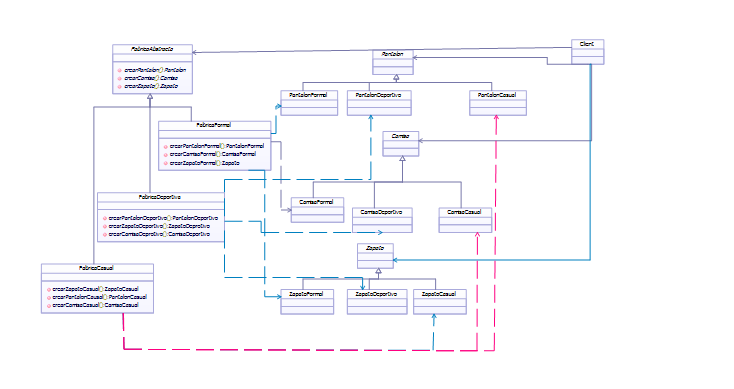
\includegraphics[width=1.2\linewidth]{arquitectura/imagenes/DiagramaFabricaAbstracta}
		\caption{Diagrama de clases Fabrica Abstracta}
	\end{figure}
	
	
	
	En el diagrama podemos ver que, para nuestro caso tendremos diferentes líneas de productos que podrán ser registrados en la base de datos. Para esto usamos el patrón fabrica abstracta que nos permite crear familias de productos de acuerdo a la línea establecida, además este patrón permite el escalamiento del aplicativo en forma horizontal, con lo cual, podremos a futuro adicionar otras nuevas líneas o colecciones de productos, sin necesidad de modificar las líneas ya creadas.
\newpage


\subsection{constructor}
\subsubsection{Modelo}
\newpage
\subsubsection{Caso}
\newpage

\subsection{Método Fábrica}
\subsubsection{Modelo}
\newpage
\subsubsection{Caso}
\newpage

\subsection{Prototipo}
\subsubsection{Modelo}
\newpage
\subsubsection{Caso}
\newpage

\section{Patrones Estructurales}

\subsection{Adaptador}
\subsubsection{Modelo}
\newpage
\subsubsection{Caso}
\newpage


\subsection{Puente}\begin{figure}[h!]
	
\subsubsection{Modelo}
\newpage
\subsubsection{Caso}
\centering
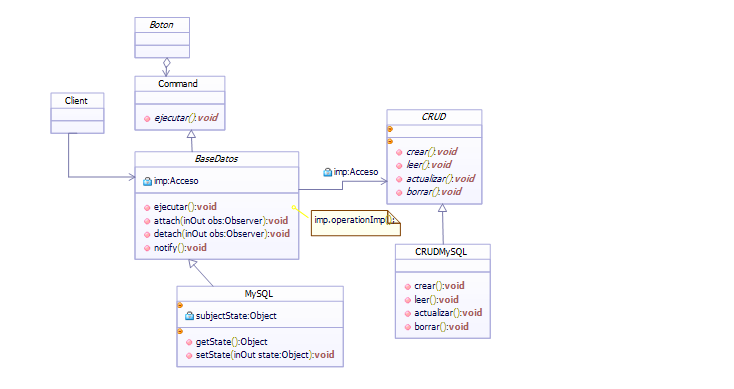
\includegraphics[width=1.0\linewidth]{arquitectura/imagenes/DiagramaComandoYPuente}
\caption{Diagrama de clases  Comando y Puente}
\end{figure}



El patrón comando utilizado en este caso permite separar y simplificar el uso de los botones y la función de cada uno en distintas opciones presentadas al usuario, para este caso particular están definidos los casos en los que el Admin crea, modifica, elimina o agrega un nuevo producto a la base de datos.
El patrón bridge, es un puente entre la abstracción de una base de datos y sus funciones con la lógica de estas funciones de acuerdo con el tipo de base de datos, puesto que la manera en que se borra, crea, agrega o modifica es diferente en cada base de datos (MySQL, Postgres, etc), de manera que en la base concreta se define el método en que cada función de la abstracción, realiza su operación. Esto permite que más adelante podamos agregar otras bases de datos a nuestro aplicativo sin la necesidad de modificar el código ya creado, y haciendo escalamiento de nuestro programa de manera horizontal.

\newpage

\subsection{componente}
\subsubsection{Modelo}
\newpage
\subsubsection{Caso}
\newpage

\subsection{Decorador}
\subsubsection{Modelo}
\newpage
\subsubsection{Caso}
\newpage

\subsection{Peso Ligero}
\subsubsection{Modelo}
\newpage
\subsubsection{Caso}
\newpage

\subsection{Proxy}
\subsubsection{Modelo}
\newpage
\subsubsection{Caso}
\newpage

\subsection{Fachada}
\subsubsection{Modelo}
\newpage
\subsubsection{Caso}
\newpage

\section{Patrones de Comportamiento}

\subsection{Comando}
\subsubsection{Modelo}
\newpage
\subsubsection{Caso}
\newpage

\subsection{Cadena de Responsabilidades}
\subsubsection{Modelo}
\newpage
\subsubsection{Caso}
\newpage

\subsection{Iterador}
\subsubsection{Modelo}
\newpage
\subsubsection{Caso}
\newpage

\subsection{Inrterprete}
\subsubsection{Modelo}
\newpage
\subsubsection{Caso}
\newpage

\subsection{Mediador}
\subsubsection{Modelo}
\newpage
\subsubsection{Caso}
\newpage

\subsection{Momento}
\subsubsection{Modelo}
\newpage
\subsubsection{Caso}
\newpage

\subsection{Observador}
\subsubsection{Modelo}
\newpage
\subsubsection{Caso}
	\begin{figure}[h!]
	\centering
	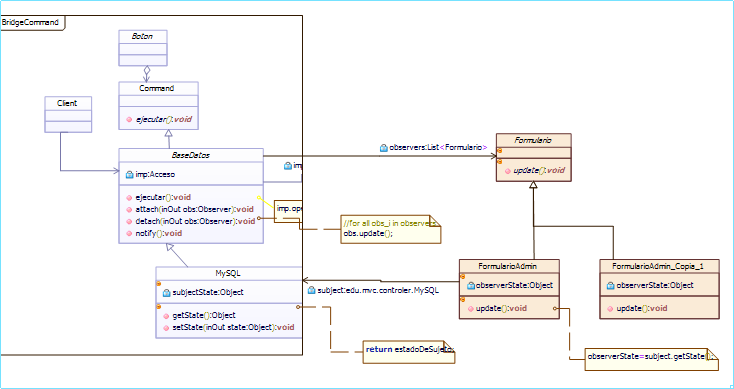
\includegraphics[width=1.0\linewidth]{arquitectura/imagenes/DiagramaObservador}
	\caption{Diagrama de clases patrón Observador}
\end{figure}



El patrón observador es utilizado en nuestro caso debido a la necesidad que tenemos de estar actualizando constantemente los datos de los productos en los formularios del Admin y el Cliente, ya sea actualizando el estado del producto en el stack, o alguna de sus características cada vez que entramos a modificarlas, este patrón nos permite facilitar esta actualización directamente en nuestra base de datos
\newpage

\newpage

\subsection{Estado}
\subsubsection{Modelo}
\newpage
\subsubsection{Caso}
\newpage

\subsection{Estrategia}
\subsubsection{Modelo}
\newpage
\subsubsection{Caso}
\newpage

\subsection{Visitador}
\subsubsection{Modelo}
\newpage
\subsubsection{Caso}
\newpage

\subsection{Método Plantilla}
\subsubsection{Modelo}
\newpage
\subsubsection{Caso}
\begin{figure}[h!]
	\centering
	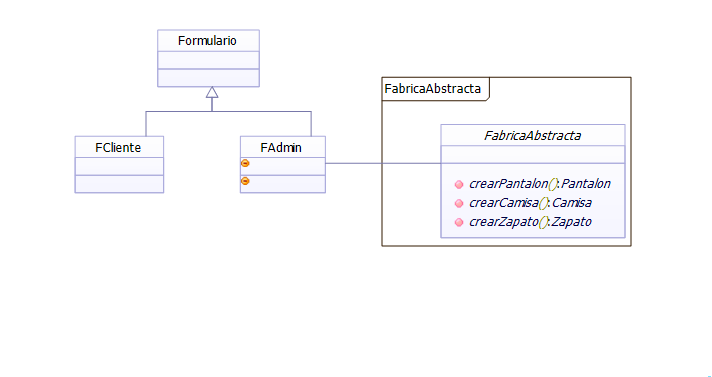
\includegraphics[width=1.0\linewidth]{arquitectura/imagenes/DiagramaFachada}
	\caption{Diagrama de clases patrón Fachada}
\end{figure}



Este patrón nos permite ocultar al cliente y al admin lo que sucede detrás del formulario que utilizan, es decir oculta la lógica del programa, la cual no es interesante para ellos, podemos incluir varios subsistemas con este patrón y dejarlos solo visibles para los realmente interesados en cada uno.

\newpage